\section{Evaluation}
\label{sec:eval}

We evaluated \kunai from three angles. First, whether the packet
structures \kunai targets can be written as filter expressions
(\S\ref{sec:eval-expr}). Second, whether the generated bytecode is
accepted by the eBPF verifier and matches/rejects as expected
(\S\ref{sec:eval-accept}). Third, the instruction count and run-time
cost of the generated bytecode (\S\ref{sec:eval-cost}).

\subsection{Method and Filter Set}
\label{sec:eval-method}

The evaluation uses ten filters, F1--F10, listed in Table~\ref{tab:filterset}. F1--F6 target basic protocol
headers such as Ethernet, VLAN, IPv4/IPv6, TCP, and ICMP, while
F7--F10 target nested headers and variable-length structures whose
start cannot be fixed at a constant offset. It lists each filter's
\kunai expression and the raw eBPF instruction count of the bytecode
\kunai generates, together with the count for the same filter compiled
from pcap-filter to eBPF through cBPF~\cite{mccanne1993bpf} using
cbpfc~\cite{cloudflare_cbpfc}, a cBPF-to-eBPF compiler. We refer to this latter count as the
pcap-filter baseline in the rest of the evaluation.

\begin{table*}[t]
  \centering\small
  \begin{tabular}{@{}llrr@{}}
    \toprule
    & & \multicolumn{2}{c}{raw insns} \\
    \cmidrule(l){3-4}
    ID & \kunai expression & \kunai & pcap-filter \\
    \midrule
    F1  & \texttt{eth/ipv4/tcp where tcp.dport == 443} & 199 & 42 \\
    F2  & \texttt{eth/ipv4[src==10.0.0.0/8]/tcp where tcp.dport == 80} & 209 & 36 \\
    F3  & \texttt{eth/ipv6[src==2001:db8::/32]/tcp} & 338 & 23 \\
    F4  & \texttt{eth/vlan[tci==100]/ipv4/tcp where tcp.dport == 80} & 215 & 51 \\
    F5  & \texttt{eth/qinq/vlan/ipv4/tcp where tcp.dport == 80} & 217 & \na \\
    F6  & \texttt{eth/ipv4/icmp where icmp.type == 8} & 85 & 31 \\
    F7  & \texttt{eth/ipv4@outer/udp/gtp/ipv4@inner/tcp where inner.dst == 10.0.0.1} & 405 & \na \\
    F8  & \texttt{eth/ipv6/srv6 where any(srv6.segments.addr == fc00::1)} & 332 & \na \\
    F9  & \texttt{eth/ipv4@outer/udp/geneve/eth/ipv4@inner/tcp where inner.dst == 10.0.0.1} & 351 & \na \\
    F10 & \texttt{eth/ipv4/tcp where tcp.options.MSS.value == 1460} & 231 & \na \\
    \bottomrule
  \end{tabular}
  \caption{Evaluation filter set and raw eBPF instruction counts.
  F7--F10 target nested headers and variable-length structures. The
  pcap-filter column is the eBPF compiled from each filter via cBPF;
  \na\ marks those pcap-filter cannot express.}
  \label{tab:filterset}
\end{table*}

To exercise the DSL syntax more broadly, we hand-constructed a separate
regression suite of 77 filter expressions, at least one per syntactic
feature of the DSL. The suite covers bracket
predicates, arithmetic in the \texttt{where} clause, quantified
layers, heterogeneous-size alternations, label disambiguation, and
aux-walks, spanning a wider syntactic range than F1--F10. Its verifier
acceptance and per-packet match/reject correctness are reported in
\S\ref{sec:eval-accept}.

To evaluate these filters, we embedded the generated bytecode in a
host BPF program and placed it at the XDP and tc attach points. The
remaining subsections use this filter set and regression suite
throughout.

\subsection{Expressiveness}
\label{sec:eval-expr}

We compared whether F1--F10 can be written in pcap-filter, the filter
language that runs in the kernel, and in \kunai. Because pcap-filter
has byte-offset access, the one expressiveness axis \kunai does
not follow (\S\ref{sec:limitations}), a hand-written
condition can sometimes be built for a specific packet layout. It does
not, however, provide as filter syntax the order of headers, an
arbitrary element of a variable-length list, repeated occurrences of
the same protocol, or a named reference to an inner header.

\textbf{Result:} F1--F6 were writable in both; only
F5 (QinQ) behaved in pcap-filter in a way that depended on the
capture environment, since NIC VLAN offload can strip the tag from the
bytes. The two diverge at F7--F10. The inner IPv4 header of F7 (GTP-U)
and F9 (Geneve) sits at no fixed offset, shifted per packet by GTP
optional fields and extension headers or by a Geneve inner Ethernet
header; F8 (SRv6) requires looping over an arbitrary segment-list
element; and F10 (TCP MSS) requires an option walk rather than a
byte-offset approximation. None of these is expressible as pcap-filter
syntax, whereas \kunai writes all of F1--F10 directly through the
labeled layer-chains, \texttt{any()}/\texttt{all()} quantifiers, and
option-field walks listed in Table~\ref{tab:filterset}.

\subsection{Verifier Acceptance and Correctness}
\label{sec:eval-accept}

We made two checks of the code generation of \S\ref{sec:codegen}:
first, that the generated bytecode is accepted by the eBPF verifier;
second, that the accepted bytecode matches and rejects as expected.

For acceptance, we loaded the bytecode generated from F1--F10 and the
regression suite onto six kernels (Linux 6.1, 6.6, 6.12, 6.15, 6.18,
7.0) at both the XDP and tc attach points. The instructions and
helpers the verifier accepts differ across kernel versions, but because
\kunai avoids version-dependent instructions as described in
\S\ref{sec:codegen}, the same bytecode was accepted unchanged on all
six versions.

At tc, the kernel extracts the outer VLAN tag into skb metadata before
the program runs. \kunai therefore rejects at compile time a filter that
reads a VLAN/QinQ field from packet bytes. An optional, predicate-free
tag stays matchable. Because at most one tag remains in the bytes,
\texttt{eth/vlan?/...} takes its skip path and matches untagged,
single-tagged, and QinQ frames without reading the stripped tag. This is
a compile-time restriction, not a verifier rejection. We excluded from
the tc loads only the field-reading forms, 2 of F1--F10 and 3 of the
regression suite, and performed 1014 loads across six kernels $\times$ 2
hosts, all accepted.

Next, we fed the generated bytecode actual packets (matching,
non-matching, and malformed) and checked the match/reject result. For
Geneve we varied \texttt{opt\_len} from 0 upward to confirm the inner
offset resolves past the skipped options, with truncated and malformed
frames throughout, and the bytecode returned the expected verdict in
every case. The regression suite was verified at two levels: all 77
expressions loaded on the verifier, and 74 of them were also checked for
match and reject correctness at the packet level; the 3 capture-clause
expressions were load-only, since their verdict equals the base chain. For the five filters both
languages express (F1 to F4 and F6) we also cross-checked \kunai against
libpcap, the engine behind tcpdump, on the same packets, and the
verdicts agreed throughout, an independent reference beyond the
hand-built expectations.

\textbf{Result:} These two checks show that the code generation of \S\ref{sec:codegen}
lowered the target filters into bytecode accepted across six kernels
$\times$ 2 hosts and traversed packet headers correctly.

\subsection{Instruction Count and Run-Time Cost}
\label{sec:eval-cost}

We first evaluate a filter's cost by the instruction count of the
generated eBPF bytecode, listed per filter in
Table~\ref{tab:filterset}. The instruction count is the static size of
the bytecode and is comparable regardless of the measurement
environment; a 64-bit immediate load is counted as two instructions
for both \kunai and pcap-filter. On the F1--F4 and F6 filters that
pcap-filter can also express, \kunai generated 2.7$\times$ to
14.7$\times$ as many instructions, the largest gap arising at the IPv6
prefix match of F3.

Because every variable-length walk is bounded at compile time, a
filter's instruction count grows with that bound, not with the packet: a
chain quantifier adds about 16 instructions per unit of cap while it
unrolls, then flattens once it lowers to a \texttt{bpf\_loop} callback,
and each stacked SRv6 segment walk, itself such a callback, adds a fixed
${\approx}68$. Even eight stacked walks stay near 800 instructions, three
orders of magnitude below the verifier's roughly one-million-instruction
limit.

To see whether this appears at run time, we connected a traffic
generator to a device under test (DUT) over 100\,GbE and attached a
native XDP program that evaluates the filter and returns
\texttt{XDP\_DROP} on every packet. The DUT runs Linux 6.15 with the
BPF JIT on an Intel Xeon 8362 and an E810 NIC. Unlike the acceptance
measurements, which cover six kernels at both the XDP and tc attach
points, the run-time figures below use this single Linux 6.15
configuration. As in an operational
fentry/tc observer, the program first copies the packet head into a
per-CPU scratch window; this copy alone lowered the rate by 6.7\%
even with no filter. We therefore measured each filter's cost as the
processing-rate reduction relative to that same-copy accept-all
baseline.

\figref{fig:datapath} shows the per-filter processing-rate reduction.
We measured at the 64-byte line rate and repeated each cell ten times;
every standard deviation was at most 0.4.

\textbf{Result:} The reduction for the basic
filters F1--F6 was 0--1.7\%, near 0\% for F6. The \kunai-only
filters F7--F10 were 3.9--7.4\%, with
F8, whose SRv6 segment list is walked by a \texttt{bpf\_loop} callback,
the largest at 7.4\%. For
F1, writable in both \kunai and pcap-filter, the difference between
the two was only 0.7\%.

\begin{figure}[htbp]
  \centering
  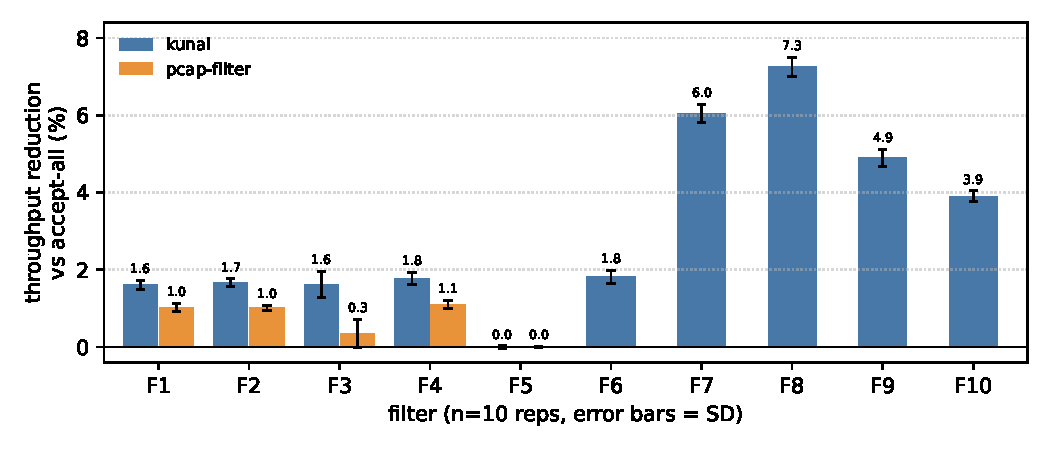
\includegraphics[width=0.62\columnwidth]{figures/fig_datapath.pdf}
  \caption{Datapath processing-rate reduction for F1--F10 (accept-all
  baseline, box plot, $n{=}10$). The heaviest filters (F7 chain walk
  6.6\%, F8 SRv6 loop 7.4\%) are comparable to the 6.7\% window-copy
  cost (dashed); triangles are means.}
  \label{fig:datapath}
\end{figure}

A per-packet run-time measurement via \texttt{BPF\_PROG\_TEST\_RUN}
agreed: over a filterless accept-all baseline of 611--612\,ns, each
filter added at most +15\,ns/pkt (under 3\%), and the
\kunai--pcap-filter difference was at most the measurement standard
deviation. Save for the SRv6 segment loop (F8), whose line-rate cost is
on par with the copy, the cost is dominated by the fixed per-packet work
every program on the datapath shares rather than by filter evaluation.
